\documentclass[12pt]{article}
\usepackage[margin=2.5cm]{geometry}
\usepackage{enumerate}
\usepackage{amsfonts}
\usepackage{amsmath}
\usepackage{fancyhdr}
\usepackage{amsmath}
\usepackage{amssymb}
\usepackage{amsthm}
\usepackage{mdframed}
\usepackage{graphicx}
\usepackage{subcaption}
\usepackage{adjustbox}
\usepackage{listings}
\usepackage{xcolor}
\usepackage{booktabs}
\usepackage[utf]{kotex}
\usepackage{hyperref}
\usepackage{accents}

\definecolor{codegreen}{rgb}{0,0.6,0}
\definecolor{codegray}{rgb}{0.5,0.5,0.5}
\definecolor{codepurple}{rgb}{0.58,0,0.82}
\definecolor{backcolour}{rgb}{0.95,0.95,0.92}

\lstdefinestyle{mystyle}{
    backgroundcolor=\color{backcolour},
    commentstyle=\color{codegreen},
    keywordstyle=\color{magenta},
    numberstyle=\tiny\color{codegray},
    stringstyle=\color{codepurple},
    basicstyle=\ttfamily\footnotesize,
    breakatwhitespace=false,
    breaklines=true,
    captionpos=b,
    keepspaces=true,
    numbers=left,
    numbersep=5pt,
    showspaces=false,
    showstringspaces=false,
    showtabs=false,
    tabsize=1
}

\lstset{style=mystyle}

\pagestyle{fancy}
\renewcommand{\headrulewidth}{0.4pt}
\lhead{CSC 343}
\rhead{Worksheet 12 Solution}

\begin{document}
\title{CSC343 Worksheet 12 Solution}
\maketitle

\begin{enumerate}[1.]
    \item

    \begin{itemize}
        \item Keys
        \begin{itemize}
            \item $\{$id of molecule$\}$
            \item $\{$x position, y position, z position$\}$
        \end{itemize}
        \item Functional Dependencies
        \begin{enumerate}[1.]
            \item id of molecule $\to$ x position, y position, z position, x velocity, y velocity, z velocity
            \item x position, y position, z position $\to$ id of molecule, x velocity, y velocity, z velocity
        \end{enumerate}
    \end{itemize}

    \bigskip

    \underline{\textbf{Notes:}}

    \bigskip

    \begin{itemize}
        \item Function Dependencies
        \begin{itemize}
            \item \textit{Functional Dependency} is a relationship between two attributes
            typically between the key and other non-key attributes within a table.

            \bigskip

            \underline{\textbf{Example:}}

            \bigskip

            $\text{SIN} \to \text{Name, Address, Birthdate}$

            \bigskip

            \underline{\textbf{Example 2:}}

            \bigskip

            $\textbf{ISBN} \to \text{Title}$

        \end{itemize}

        \item Key of Relations
        \begin{itemize}
            \item One or more attributes $\{A_1,A_2,...,A_n\}$ is a key for a relation R if
            \begin{enumerate}[1.]
                \item Those attributes functionally determine all other attributes of the relation
                \item No proper subset of $\{A_1,A_2,...A_n\}$ functionally determines all other attributes of R


                \bigskip

                \underline{\textbf{Example:}}

                \bigskip

                Given relation

                \bigskip

                $R = \text{Movies1(title, year, length, genre, studioName, starName)}$

                \begin{enumerate}
                    \item $\{$title, year, starName $\}$ form a key for the relation \textbf{Movies1}
                    \item $\{$ year, starName $\}$ is not a key. Same star can be in multiple
                    movies per year
                \end{enumerate}
            \end{enumerate}

            \item Superkeys
            \begin{itemize}
                \item Means a a set of attributes that contains a key
                \item Don't need to be minimal

                \bigskip

                \underline{\textbf{Example:}}

                Given relation

                \bigskip

                $R = \text{Movies1(title, year, length, genre, studioName, starName)}$

                \begin{itemize}
                    \item $\{$ title, year, starName $\}$ is a key and superkey
                    \item $\{$ title, year, starName, title, year, length$\}$ is a superkey
                \end{itemize}
            \end{itemize}
        \end{itemize}
    \end{itemize}

    \bigskip

    \underline{\textbf{References:}}

    \bigskip

    \begin{enumerate}[1)]
        \item OpenTextBC, Chapter 11 Functional Dependencies, \href{https://opentextbc.ca/dbdesign01/chapter/chapter-11-functional-dependencies/#:~:text=A%20functional%20dependency%20(FD)%20is,determines%20the%20value%20of%20Y.}{link}
    \end{enumerate}

    \item

    \begin{enumerate}[a)]

        \item

        \begin{enumerate}[1.]
            \item $AB \to C$
            \item $AB \to D$
            \item $C \to A$
            \item $C \to B$
            \item $D \to B$
            \item $D \to C$
            \item $C \to D$
            \item $D \to A$
        \end{enumerate}

        \bigskip

        \begin{mdframed}
            \underline{\textbf{Second Attempt:}}

        $\{A,B\}^+ = \{A,B,C,D\}$, so the following non-trivial FDs follows:
        $AB \to C$ and $AB \to D$.

        \bigskip

        $\{C\}^+ = \{D,A\}$, so the following non-trivial FDs follows
        $C \to D$ and $C \to A$.

        \bigskip
        $\{D\}^+ = \{A\}$, so the following non-trivial FDs follows:
        $D \to A$.


        \end{mdframed}

        \bigskip

        \underline{\textbf{Notes:}}

        \bigskip

        \begin{itemize}
            \item The Splitting / Combining Rule
            \begin{itemize}
                \item Combining Rule
                \begin{itemize}
                    \item

                    $A_1,A_2,\cdots,A_n \to B_i$ for $i = 1,2,...,m$

                    to

                    $A_1,A_2,\cdots A_n \to B_1,B_2,\cdots B_m$
                \end{itemize}

                \bigskip

                \underline{\textbf{Example:}}

                \bigskip

                Given

                \bigskip

                title year $\to$ length

                title year $\to$ genre

                title year $\to$ studioName

                \bigskip

                it's combined form is

                \bigskip

                title year $\to$ length genre studioName

                \bigskip

                \item Splitting Rule
                \begin{itemize}
                    \item
                    \item

                    $A_1,A_2,\cdots A_n \to B_1,B_2,\cdots B_m$

                    to

                    $A_1,A_2,\cdots,A_n \to B_i$ for $i = 1,2,...,m$

                \end{itemize}

                \bigskip

                \underline{\textbf{Example:}}

                \bigskip

                Given

                \bigskip

                title year $\to$ length

                \bigskip

                It's splitted form is

                \bigskip

                title $\to$ length

                year $\to$ length
            \end{itemize}

            \item Trivial Functional Dependencies

            \bigskip

            \begin{itemize}
                \item A functional dependency $FD: X \to Y$ is \textbf{trivial}
                if $Y$ is a subset of $X$

                \bigskip

                \underline{\textbf{Exmaple:}}

                \bigskip

                title year $\to$ title

                \bigskip

                \underline{\textbf{Example 2:}}

                \bigskip

                title $\to$ title

            \end{itemize}

            \item Non-trivial Functional Dependencies
            \begin{itemize}
                \item is a case where some but not all of the attributes on the R.H.S
                of an FD are also on L.H.S

                \bigskip

                \underline{\textbf{Example:}}

                \bigskip

                title year $\to$ title movieLength

                \bigskip

                \item Can be simplified using \textbf{tirivial-dependency rule}
                \begin{itemize}
                    \item The $FD$ $A_1A_2 \cdots A_n \to B_1B_2 \cdots B_m$ is equivalent to

                    $A_1 A_2 \cdots A_n \to C_1 C_2 \cdots C_k$

                    \bigskip

                    where $C$'s are all those $B$'s that are not in $A$'s.


                    \begin{center}
                    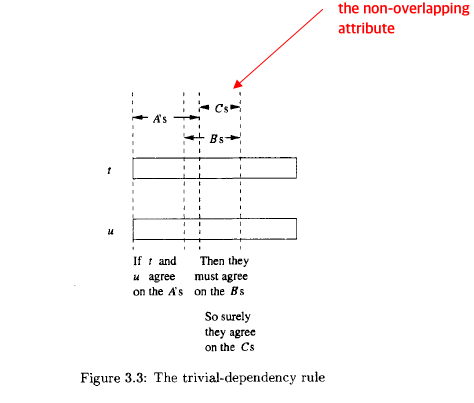
\includegraphics[width=\linewidth]{images/worksheet_12_solution_1.png}
                    \end{center}
                \end{itemize}
            \end{itemize}

            \item Computing the Clousre of Attributes
            \begin{itemize}
                \item Closure of attribute set $\{X\}$ is denoted as $\{X\}^+$.
                \item The closure means a given set of attributes $A$ satisfying FD, are a sets of all attributes
                $B$ such that $A \to B$

                \bigskip

                \underline{\textbf{Example:}}

                \bigskip


                Given attributes $A,B,C,D,E,F$ and FDs $AB \to C$, $BC \to AD$, $D \to E$
                and $CF \to B$, What is the closure of $\{A,B\}$ or $\{A,B\}^+$

                \bigskip

                \begin{enumerate}[1.]
                    \item Start with $\{A,B\}$.
                    \item Split $BC \to AD$
                    \begin{itemize}
                        \item We have $BC \to A$ and $BC to D$
                        \item Since $A$ is in $\{A,B\}$, this is not included
                        \item Since $D$ is not in  $\{A,B\}$, this IS included

                        \bigskip

                        So, we have $\{A,B,D\}$
                    \end{itemize}
                    \item Since $C$ in $AB \to C$ is NOT in $\{A,B,C,D\}$, $C$ is included and we have $\{A,B,C,D\}$
                    \item Since $A$ in $BC \to A$ is in $\{A,B,C,D\}$, this is skipped
                    \item Since $E$ is not in $D \to E$, $E$ is included and we have $\{A,B,C,D,E\}$
                    as our solution
                \end{enumerate}
            \end{itemize}

            \item Why the Closure Algorithm Works
            \item Transitive Rule
            \begin{itemize}
                \item Definition

                \bigskip

                If $A_1A_2 \cdots A_n \to B_1B_2 \cdots B_m$ and $B_1B_2 \cdots B_m \to C_1C_2 \cdots C_k$
                hold in relation $R$, $A_1A_2 \cdots A_n \to C_1C_2 \cdots C_k$ also holds in $R$.

                \bigskip

                \underline{\textbf{Example:}}

                \bigskip

                Given

                \bigskip

                title year $\to$ studioName

                studioName $\to$ studioAddr

                \bigskip

                Transitive rule says the above is equal to the following

                \bigskip

                title year $\to$ studioAddr

            \end{itemize}

            \item Inference Rules
            \begin{itemize}
                \item Is allso called \textbf{Armstrong's Axioms}
                \item Has 3 axioms
                \begin{enumerate}[1.]
                    \item \textit{Reflexivity}
                    \begin{itemize}
                        \item If $\{B_1, B_2, ..., B_n\} \subseteq \{A_1, A_2, ..., A_n\}$ then

                        $A_1A_2 \cdots  A_n \to B_1B_2 \cdots B_m$
                        \item also called \textbf{trivial FDs}
                    \end{itemize}
                    \item \textit{Augmentation}
                    \begin{itemize}
                        \item If $A_1A_2 \cdots A_n \to B_1B_2 \cdots B_m$

                        then $A_1A_2 \cdots A_nC_1C_2 \cdots C_k \to B_1B_2 \cdots B_m C_1C_2 \cdots C_k$

                        \item $ C_1C_2 \cdots C_k$ are any set of attributes
                    \end{itemize}
                    \item \textit{Transitivity}
                    \begin{itemize}
                        \item If $A_1A_2 \cdots A_n \to B_1B_2 \cdots B_m$ and $B_1B_2 \cdots B_m \to C_1C_2 \cdots C_k$

                        then $A_1A-2 \cdots A_n \to C_1C_2 \cdots C_k$

                    \end{itemize}
                \end{enumerate}
            \end{itemize}
        \end{itemize}

        \item

        ${A,B}$ is the only key of $R$.

        \bigskip

        \underline{\textbf{Notes:}}

        \bigskip

        \begin{itemize}
            \item Key of Attributes
            \begin{itemize}
                \item \textbf{Definition:} A set of attributes $\{A_1,A_2,\cdots,A_n\}$
                is a key for a relation $R$ if


                \begin{enumerate}[1.]
                    \item Those attributes functionally determine all other attributes
                    \item No proper subset of $\{A_1, A_2, ..., A_n\}$ functionally determines all other attributes
                    of $R$.
                \end{enumerate}
            \end{itemize}
        \end{itemize}

        \item

        The superkeys that are not keys are: $\{A,B,C\}$, $\{A,B,D\}$, $\{A,B,C,D\}$
    \end{enumerate}

    \item

    \begin{enumerate}[i)]
        \item

        \begin{enumerate}[a)]
            \item

            \bigskip

            $\{A\}^+ = \{A,B,C,D\}$, so we have $A \to A$, $A \to B$, $A \to C$, $A \to D$

            \bigskip

            $\{B\}^+ = \{C,D\}$, so we have $B \to C$ and $B \to D$

            \item

            $\{A\}$ is the key of $S$.

            \item

            The super keys that are not keys are:

            \bigskip

            $\{A,B\}$, $\{A,C\}$, $\{A,D\}$, $\{A,B,C\}$, $\{A,B,D\}$, $\{A,B,C,D\}$
        \end{enumerate}

        \item

        \begin{enumerate}[a)]
            \item

            \bigskip

            $\{A\}^+ = \{A\}$, so this FD is trivial.

            \bigskip

            $\{B\}^+ = \{B\}$, so this FD is trivial.

            \bigskip

            $\{C\}^+ = \{C\}$, so this FD is trivial.

            \bigskip

            $\{D\}^+ = \{D\}$, so this FD is trivial.

            \bigskip

            $\{A,B\}^+ = \{A,B,C,D\}$, so we have $AB \to A$, $AB \to B$, $AB \to C$, $AB \to D$

            \bigskip

            $\{A,C\}^+ = \{A,C\}$, so we have $AC \to A$, $AC \to C$

            \bigskip

            $\{A,D\}^+ = \{A,D,B\}$, so we have $AD \to A$, $AD \to D$, $AD \to B$

            \bigskip

            $\{B,C\}^+ = \{B,C,D,A\}$, so we have $BC \to A$, $BC \to B$, $BC \to C$, $BC \to D$

            \bigskip

            $\{D,C\}^+ = \{D,C,A,B\}$, so we have $DC \to D$, $DC \to C$, $DC \to A$, $DC \to B$

            \bigskip

            $\{A,B,C\}^+ = \{A,B,C,D\}$, so we have $ABC \to A$, $ABC \to B$, $ABC \to C$, $ABC \to D$

            \bigskip

            $\{B,C,D\}^+ = \{B,C,D,A\}$, so we have $BCD \to A$, $BCD \to B$, $BCD \to C$, $BCD \to D$

            \bigskip

            $\{C,D,A\}^+ = \{C,D,A,B\}$, so we have $CDA \to A$, $CDA \to B$, $CDA \to C$, $CDA \to D$

            \bigskip

            $\{D,A,B\}^+ = \{D,A,B,C\}$, so we have $DAB \to A$, $DAB \to B$, $DAB \to C$, $DAB \to D$

            \bigskip

            $\{D,A,B\}^+ = \{D,A,B,C\}$, so we have $DAB \to A$, $DAB \to B$, $DAB \to C$, $DAB \to D$

            \bigskip

            $\{A,B,C,D\}^+ = \{A,B,C,D\}$, so this FD is trivial.

            \item

            $\{A,B\}$, $\{A,C\}$, $\{B,C\}$, $\{D,C\}$ are the keys of $T$.

            \bigskip

            \item

            The super keys that are not keys are:

            \bigskip

            $\{A,B,C\}$, $\{A,B,D\}$, $\{B,C,D\}$, $\{A,D,C\}$, $\{A,B,D\}$, $\{A,B,C,D\}$

        \end{enumerate}

        \item

        \begin{enumerate}[a)]
            \item

            $\{A\}^+ = \{A,B,C,D\}$, so we have $A \to C$, $A \to D$

            \bigskip

            $\{B\}^+ = \{A,B,C,D\}$, so we have $B \to A$, $B \to D$

            \bigskip

            $\{C\}^+ = \{A,B,C,D\}$, so we have $C \to A$, $C \to B$

            \bigskip

            $\{D\}^+ = \{A,B,C,D\}$, so we have $D \to B$, $D \to C$

            \bigskip

            $\{A,B\}^+ = \{A,B,C,D\}$, so we have $AB \to C$, $AB \to D$

            \bigskip

            $\{B,C\}^+ = \{A,B,C,D\}$, so we have $BC \to A$, $BC \to D$

            \bigskip

            $\{B,D\}^+ = \{A,B,C,D\}$, so we have $BD \to A$, $BD \to C$

            \bigskip

            $\{C,D\}^+ = \{A,B,C,D\}$, so we have $CD \to A$, $CD \to B$

            \bigskip

            $\{C,D\}^+ = \{A,B,C,D\}$, so we have $CD \to A$, $CD \to B$

            \bigskip

            $\{A,B,C\}^+ = \{A,B,C,D\}$, so we have $ABC \to D$

            \bigskip

            $\{B,C,D\}^+ = \{A,B,C,D\}$, so we have $BCD \to A$

            \bigskip

            $\{C,D,A\}^+ = \{A,B,C,D\}$, so we have $CDA \to B$

            \bigskip

            $\{D,A,B\}^+ = \{A,B,C,D\}$, so we have $DAB \to C$

            \bigskip

            \begin{mdframed}
                \underline{\textbf{Correct Solution:}}

                $\{A\}^+ = \{A,B,C,D\}$, so we have $A \to C$, $A \to D$

                \bigskip

                $\{B\}^+ = \{A,B,C,D\}$, so we have $B \to A$, $B \to D$

                \bigskip

                $\{C\}^+ = \{A,B,C,D\}$, so we have $C \to A$, $C \to B$

                \bigskip

                $\{D\}^+ = \{A,B,C,D\}$, so we have $D \to B$, $D \to C$

                \bigskip

                $\{A,B\}^+ = \{A,B,C,D\}$, so we have $AB \to C$, $AB \to D$

                \bigskip

                \color{red}$\{A,C\}^+ = \{A,B,C,D\}$, so we have $AC \to B$, $AC \to D$\color{black}

                \bigskip

                \color{red}$\{A,D\}^+ = \{A,B,C,D\}$, so we have $AD \to B$, $AD \to C$\color{black}

                \bigskip

                $\{B,C\}^+ = \{A,B,C,D\}$, so we have $BC \to A$, $BC \to D$

                \bigskip

                $\{B,D\}^+ = \{A,B,C,D\}$, so we have $BD \to A$, $BD \to C$

                \bigskip

                $\{C,D\}^+ = \{A,B,C,D\}$, so we have $CD \to A$, $CD \to B$

                \bigskip

                $\{A,B,C\}^+ = \{A,B,C,D\}$, so we have $ABC \to D$

                \bigskip

                $\{B,C,D\}^+ = \{A,B,C,D\}$, so we have $BCD \to A$

                \bigskip

                $\{C,D,A\}^+ = \{A,B,C,D\}$, so we have $CDA \to B$

                \bigskip

                $\{D,A,B\}^+ = \{A,B,C,D\}$, so we have $DAB \to C$

            \end{mdframed}

            \bigskip

            \item

            $\{A\},\{B\},\{C\},\{D\}$ are the keys of $U$.

            \item

            The super keys that are not keys are:

            \bigskip

            $\{A,B\}$,$\{A,C\}$,$\{A,D\}$,$\{B,C\}$, $\{B,D\}$,$\{C,D\}$, $\{A,B,C\}$,
            $\{B,C,D\}$, $\{C,D,A\}$, $\{D,A,B\}$. $\{A,B,C,D\}$

        \end{enumerate}

    \end{enumerate}

    \item

        \begin{enumerate}[a)]
            \item

            We need to show the closure of attributes $\{A_1,A_2,\cdots,A_n,C\}$ in
            \\ $FD$ $A_1,A_2,\cdots,A_n,C \to B$ is $\{A_1,A_2,\cdots,A_n,C,B\}$, that is
            $\{A_1,A_2,\cdots,A_n,C\}^+ = \{A_1,A_2,\cdots,A_n,C,B\}$

            \bigskip

            Since we know $\{A_1,A_2,\cdots,A_n\}$ functionally determines $B$,
            we can conclude $B$ can be added to $\{A_1,A_2,\cdots,A_n,C\}$.

            \bigskip

            Thus, it follows from above that $\{A_1,A_2,\cdots,A_n,C\}^+ = \{A_1,A_2,\cdots,A_n,C,B\}$.

            \item

            Let $A_1A_2\cdots A_n \to B$ is FD. That is, $\{A_1A_2\cdots A_n\}^+ = \{A_1A_2\cdots A_n, B\}$

            \bigskip

            We need to show $A_1A_2 \cdots A_nC \to BC$ follows. That is,
            $\{A_1,A_2,\cdots,A_n,C\}^+ = \{A_1,A_2,\cdots,A_n,C,B\}$

            \bigskip

            It follows from the combine and split rule that $A_1A_2\cdots A_n C \to BC$
            can be spliited into $A_1A_2\cdots A_nC \to B$ and $A_1A_2\cdots,A_nC \to C$.

            \bigskip

            So, we need to show $A_1A_2\cdots A_nC \to B$ and $A_1A_2\cdots,A_nC \to C$ follows
            from the given.

            \bigskip

            We will do so in parts.

            \bigskip

            \begin{enumerate}[1.]
                \item \textbf{Part 1 (Showing $A_1A_2\cdots A_nC \to B$):}

                \bigskip

                Here, we need to show $A_1A_2\cdots A_nC \to B$ follows.

                \bigskip

                And indeed, this follows from the work of \textit{augmenting left sides}.
                That is the solution to previous problem.

                \bigskip

                \item \textbf{Part 2 (Showing $A_1A_2 \cdots A_nC \to C$):}

                \bigskip

                Here, we need to show $A_1A_2 \cdots A_nC \to C$ follows.

                \bigskip

                The definition of trivial FD tells us $A_1A_2 \cdots A_n \to B_1B_2 \cdots B_m$
                holds when\\ $\{B_1,B_2,\cdots,B_m\} \subseteq \{A_1,A_2,\cdots,A_n\}$

                \bigskip

                Since $\{C\} \subseteq \{A_1,A_2\cdots,A_n,C\}$, we can conclude
                this FD follows trivially.

            \end{enumerate}


            % \begin{mdframed}

            %     \underline{\textbf{Rough Work:}}

            %     Let $A_1A_2\cdots A_n \to B$ is FD. That is, $\{A_1A_2\cdots A_n\}^+ = \{A_1A_2\cdots A_n, B\}$

            %     \bigskip

            %     We need to show $A_1A_2 \cdots A_nC \to BC$ follows. That is,
            %     $\{A_1,A_2,\cdots,A_n,C\}^+ = \{A_1,A_2,\cdots,A_n,C,B\}$


            %     \bigskip

            %     \begin{enumerate}[1.]
            %         \item Use the split rule to split $A_1A_2\cdots A_n C \to BC$
            %         into $A_1A_2\cdots A_nC \to B$ and $A_1A_2\cdots,A_nC \to C$

            %         \begin{mdframed}
            %         It follows from the combine and split rule that $A_1A_2\cdots A_n C \to BC$
            %         can be spliited into $A_1A_2\cdots A_nC \to B$ and $A_1A_2\cdots,A_nC \to C$.

            %         \bigskip

            %         So, we need to show $A_1A_2\cdots A_nC \to B$ and $A_1A_2\cdots,A_nC \to C$ follows
            %         from the given.

            %         \bigskip

            %         We will do so in parts.
            %         \end{mdframed}

            %         \item Prove $A_1A_2\cdots A_nC \to B$ and $A_1A_2\cdots,A_nC \to C$
            %         in parts
            %         \begin{enumerate}[1)]
            %             \item Show $A_1A_2\cdots A_nC \to B$ follows

            %             \begin{mdframed}
            %             We can conclude this holds by the work of \textit{augmenting left sides}.
            %             That is the solution to previous problem.
            %             \end{mdframed}

            %             \item Show $A_1A_2\cdots,A_nC \to C$ follows

            %             \begin{mdframed}
            %             The definition of trivial FD tells us $A_1A_2 \cdots A_n \to B_1B_2 \cdots B_m$
            %             is trivial when $\{B_1,B_2,\cdots,B_m\} \subseteq \{A_1,A_2,\cdots,A_n\}$

            %             \bigskip

            %             Since $\{C\} \subseteq \{A_1,A_2\cdots,A_n,C\}$, we can conclude
            %             this FD follows trivially.
            %             \end{mdframed}
            %         \end{enumerate}
            %     \end{enumerate}

            % \end{mdframed}

            \item

            Let $A_1A_2 \cdots A_n \to B_1B_2 \cdots B_m$ and $C_1C_2 \cdots C_k \to D$,
            where $B$ are each among the $C$'s.

            \bigskip

            We neeed to show $A_1A_2\cdots A_n E_1E_2 \cdots E_j \to D$ follows,
            where the $E$'s are all of those $C$'s not found among the $B$'s.

            \bigskip

            The transitive rule tells us if $A_1A_2\cdots A_n \to B_1B_2 \cdots B_m$
            and $B_1B_2 \cdots B_m \to C_1 C_2 \cdots C_k$, then $A_1A_2 \cdots A_n \to C_1 C_2 \cdots C_k$
            also holds in $R$.

            \bigskip

            Since we know $A_1A_2 \cdots A_n \to B_1B_2 \cdots B_m$ and $C_1C_2 \cdots C_k \to D$
            where $B$'s are each among the $C$'s, we can conclude from the transitive rule
            that $A_1A_2 \cdots A_n \to D$.

            \bigskip

            Then using \textbf{augmenting left sides} to all $C$'s not found among the $B$'s
            on $A_1 A_2 \cdots A_n \to D$, we can conclude $A_1A_2 \cdots A_n E_1 E_2 \cdots E_j \to D$ follows.


            \bigskip


            % \underline{\textbf{Rough Work:}}

            % \bigskip

            % Let $A_1A_2 \cdots A_n \to B_1B_2 \cdots B_m$ and $C_1C_2 \cdots C_k \to D$,
            % where $B$ are each among the $C$'s.

            % \bigskip

            % We neeed to show $A_1A_2\cdots A_n E_1E_2 \cdots E_j \to D$ follows,
            % where the $E$'s are all of those $C$'s not found among the $B$'s.

            % \bigskip


            % \begin{enumerate}[1.]
            %     \item Show using transitive rule that $A_1 A_2 \cdots A_n \to D$ holds.

            %     \begin{mdframed}
            %     The transitive rule tells us if $A_1A_2\cdots A_n \to B_1B_2 \cdots B_m$
            %     and $B_1B_2 \cdots B_m \to C_1 C_2 \cdots C_k$, then $A_1A_2 \cdots A_n \to C_1 C_2 \cdots C_k$
            %     also holds in $R$.

            %     \bigskip

            %     Since we know $A_1A_2 \cdots A_n \to B_1B_2 \cdots B_m$ and $C_1C_2 \cdots C_k \to D$
            %     where $B$'s are each among the $C$'s, we can conclude from the transitive rule
            %     that $A_1A_2 \cdots A_n \to D$.

            %     \end{mdframed}

            %     \item Show using Augmenting Left Sides that $A_1 A_2 \cdots A_n E_1 E_2 \cdots E_n \to D$ follows
            %     follows

            %     \begin{mdframed}
            %     Then using \textbf{augmenting left sides} to all $C$'s not found among the $B$'s
            %     on $A_1 A_2 \cdots A_n \to D$, we can conclude $A_1A_2 \cdots A_n E_1 E_2 \cdots E_j \to D$ follows.

            %     \end{mdframed}

            %     \bigskip

            % \end{enumerate}

            \item

            Assume $FD$'s $A_1A_2 \cdots A_n \to B_1 B_2 \cdots B_m$ and $C_1 C_2 \dots C_k \to D_1 D_2 \cdots D_j$ holds.

            \bigskip

            We need to show $FD$ $A_1A_2 \cdots A_n C_1 C_2 \cdots C_k \to B_1 B_2 \cdots B_m D_1 D_2 \cdots D_k$ follows.

            \bigskip

            Using the split / combine rule, we can conclude showing $A_1A_2 \cdots A_n C_1 C_2 \cdots C_k \to B_1 B_2 \cdots B_m D_1 D_2 \cdots D_k$ is
            the same as showing $A_1A_2 \cdots A_n C_1 C_2 \cdots C_k \to B_1 B_2 \cdots B_m$ and
            $A_1A_2 \cdots A_n C_1 C_2 \cdots C_k \to D_1 D_2 \cdots D_k$

            \bigskip

            So, we will prove the two, in parts

            \bigskip

            \begin{enumerate}[1.]
                \item \textbf{Part 1 (Showing $A_1A_2 \cdots A_n C_1 C_2 \cdots C_k \to B_1 B_2 \cdots B_m$)}

                \bigskip

                Here, we need to show $A_1A_2 \cdots A_n C_1 C_2 \cdots C_k \to B_1 B_2 \cdots B_m$.

                \bigskip

                The header of problem tells us $A_1A_2 \cdots A_n \to B_1 B_2 \cdots B_m$ holds.

                \bigskip

                Then by using \textbf{Augmenting Left Sides} rule to all $C$s not
                found among the $A$s, $A_1A_2 \cdots A_n C_1 C_2 \cdots C_k \to B_1 B_2 \cdots B_m$ follows.

                \bigskip

                \item \textbf{Part 2 (Showing $A_1A_2 \cdots A_n C_1 C_2 \cdots C_k \to D_1 D_2 \cdots D_k$ follows)}

                \bigskip

                Here, we need to show $A_1A_2 \cdots A_n C_1 C_2 \cdots C_k \to D_1 D_2 \cdots D_k$.

                \bigskip

                The header of problem tells us $C_1 C_2 \cdots C_k \to D_1 D_2 \cdots D_k$ holds.

                \bigskip

                Then by using \textbf{Augmenting Left Sides} rule to all $A$s not
                found among the $C$s, $A_1A_2 \cdots A_n C_1 C_2 \cdots C_k \to D_1 D_2 \cdots D_k$ follows.

            \end{enumerate}

            \bigskip

            % \underline{\textbf{Rough Work:}}

            % \bigskip

            % Assume $FD$'s $A_1A_2 \cdots A_n \to B_1 B_2 \cdots B_m$ and $C_1 C_2 \dots C_k \to D_1 D_2 \cdots D_j$ holds.

            % \bigskip

            % We need to show $FD$ $A_1A_2 \cdots A_n C_1 C_2 \cdots C_k \to B_1 B_2 \cdots B_m D_1 D_2 \cdots D_k$ follows.

            % \bigskip

            % \begin{enumerate}[1.]
            %     \item Using split combine rule, split $A_1A_2 \cdots A_n C_1 C_2 \cdots C_k \to B_1 B_2 \cdots B_m D_1 D_2 \cdots D_k$
            %     into $A_1A_2 \cdots A_n C_1 C_2 \cdots C_k \to B_1 B_2 \cdots B_m$ and  $A_1A_2 \cdots A_n C_1 C_2 \cdots C_k \to D_1 D_2 \cdots D_k$

            %     \bigskip

            %     \begin{mdframed}
            %     The split / combine rule tells us showing $A_1A_2 \cdots A_n C_1 C_2 \cdots C_k \to B_1 B_2 \cdots B_m D_1 D_2 \cdots D_k$ is
            %     the same as showing $A_1A_2 \cdots A_n C_1 C_2 \cdots C_k \to B_1 B_2 \cdots B_m$ and
            %     \\ $A_1A_2 \cdots A_n C_1 C_2 \cdots C_k \to D_1 D_2 \cdots D_k$

            %     \bigskip

            %     So, we will prove the two, in parts

            %     \end{mdframed}

            %     \bigskip

            %     \begin{enumerate}[1.]
            %         \item Show $A_1A_2 \cdots A_n C_1 C_2 \cdots C_k \to B_1 B_2 \cdots B_m$ follows

            %         \begin{mdframed}
            %         Here, we need to show $A_1A_2 \cdots A_n C_1 C_2 \cdots C_k \to B_1 B_2 \cdots B_m$ follows.

            %         \bigskip

            %         The header of problem tells us $A_1A_2 \cdots A_n \to B_1 B_2 \cdots B_m$ holds.

            %         \bigskip

            %         Then by using \textbf{Augmenting Left Sides} rule to all $C$s not
            %         found among the $A$s, $A_1A_2 \cdots A_n C_1 C_2 \cdots C_k \to B_1 B_2 \cdots B_m$ follows.


            %         \end{mdframed}
            %         \item Show $A_1A_2 \cdots A_n C_1 C_2 \cdots C_k \to D_1 D_2 \cdots D_k$ follows

            %         \begin{mdframed}
            %         Here, we need to show $A_1A_2 \cdots A_n C_1 C_2 \cdots C_k \to D_1 D_2 \cdots D_k$ follows.

            %         \bigskip

            %         The header of problem tells us $C_1 C_2 \cdots C_k \to D_1 D_2 \cdots D_k$ holds.

            %         \bigskip

            %         Then by using \textbf{Augmenting Left Sides} rule to all $A$s not
            %         found among the $C$s, $A_1A_2 \cdots A_n C_1 C_2 \cdots C_k \to D_1 D_2 \cdots D_k$ follows.


            %         \end{mdframed}
            %     \end{enumerate}
            % \end{enumerate}

        \end{enumerate}

        \item

        \begin{enumerate}[a)]
            \item

            An example is

            \bigskip

            $A$ being movieID and

            $B$ being movie length.

            \item

            An example is

            \bigskip

            $A$ being movieID

            $B$ being movieTitle

            $C$ being movieLength

            \item

            An example is

            \bigskip

            $A$ being movieTitle

            $B$ being year

            $C$ being length
        \end{enumerate}

        \item

        \bigskip

        Assume a relation has no attribute that is functionallty determined
        by all the other attributes.

        \bigskip

        And, assume for the sake of contradiction that there is a relation with
        non-trivial FD $X \to Y$.

        \bigskip

        Then, it follows from the definition of non-trivial functional dependency
        that $Y \neq\subseteq X$.

        \bigskip

        Then, we can conclude the attributes in $Y$ is functionally determined by other
        attributes in $X$.

        \bigskip

        But this contradicts the assumption that no attribute is functionally
        determined by all other attributes.

        \bigskip

        % \begin{mdframed}
        %     \underline{\textbf{Rough Work:}}

        %     Assume a relation has no attribute that is functionallty determined
        %     by all the other attributes.

        %     \bigskip

        %     And, assume for the sake of contradiction that there is a relation with
        %     non-trivial FD $X \to Y$.

        %     \bigskip

        %     Then, it follows from the definition of non-trivial functional dependency
        %     that $Y \neq\subseteq X$.

        %     \bigskip

        %     Then, we can conclude the attributes in $Y$ is functionally determined by other
        %     attributes in $X$.

        %     \bigskip

        %     But this contradicts the assumption that no attribute is functionally
        %     determined by all other attributes.

        % \end{mdframed}

        \item

        Let $X$ and $Y$ be sets of attributes. Assume $X \subseteq Y$.

        \bigskip

        I need to show $X^+ \subseteq Y^+$.

        \bigskip

        I will do so in cases

        \begin{enumerate}[1.]
            \item \textbf{Case 1 ($X = Y$):}

            \bigskip

            Assume $X = Y$.

            \bigskip

            I need to show $X^+ \subseteq Y^+$ follows.

            \bigskip

            The header tells us $X = Y$.

            \bigskip

            Using this fact, $X^+ = Y^+$ is true.

            \bigskip

            Then it follows from above that $X^+ \subseteq Y^+$ is also true.

            \item \textbf{Case 2 ($X \subset Y$)}

            \bigskip

            Assume $X \subset Y$.

            \bigskip

            I need to show $X^+ \subseteq Y^+$ follows.

            \bigskip

            Since the attributes in $X$ is in $Y$, we can conclude the attributes in $X^+$
            is also in $Y^+$.

            \bigskip

            And, since $Y$ has attributes not in $X$, we can conclude $Y^+$ may
            contain attributes not in $X^+$.

            \bigskip

            Thus, we can conclude $X^+ \subseteq Y^+$.

        \end{enumerate}

        % \underline{\textbf{Rough Work:}}

        % \bigskip

        % Let $X$ and $Y$ be sets of attributes. Assume $X \subseteq Y$.

        % \bigskip

        % I need to show $X^+ \subseteq Y^+$.

        % \bigskip

        % I will do so in cases

        % \begin{enumerate}[1.]
        %     \item Case where $X = Y$
        %     \begin{enumerate}[1.]
        %         \item Show that all attributes in $Y^+$ includes all attributes from $X^+$

        %         \begin{mdframed}
        %         Since $X = Y$, we can write $X^+ = Y^+$.
        %         \end{mdframed}

        %         \item Conclude $X^+ \subseteq Y^+$

        %         \begin{mdframed}
        %         Then it follows from above that $X^+ \subseteq Y^+$ is also true.
        %         \end{mdframed}
        %     \end{enumerate}

        %     \item Case where $X \subset Y$
        %     \begin{enumerate}[1.]
        %         \item Show that all attributes in $Y^+$ includes all attributes from $X^+$
        %         in addition to attributes not in $X^+$.

        %         \begin{mdframed}
        %         Since attributes in $X$ is in $Y$, we can conclude the attributes in $X^+$
        %         is also in $Y^+$.

        %         \bigskip

        %         And, since $Y$ has attributes not in $X$, we can conclude $Y^+$ may
        %         contain attributes not in $X^+$.
        %         \end{mdframed}

        %         \item Conclude $X^+ \subseteq Y^+$.

        %         \begin{mdframed}
        %         Thus, we can conclude $X^+ \subseteq Y^+$.
        %         \end{mdframed}
        %     \end{enumerate}
        % \end{enumerate}

        \item

        \begin{enumerate}[1.]
            \item Only one solution will be included for now :)

            The following

            \begin{enumerate}[1.]
                \item $A \to C$
                \item $B \to A$
                \item $B \to C$
                \item $C \to A$
                \item $C \to B$
                \item $AB \to C$
                \item $AC \to B$
                \item $BC \to A$
                \item $A \to BC$
                \item $A \to A$
            \end{enumerate}

            can be simplified to

            \begin{enumerate}[1.]
                \item $A \to C$
                \item $B \to A$
                \item $B \to C$
                \item $C \to A$
                \item $C \to B$
                \item $A \to C$ \color{red}B removed from here!!\color{black}
                \item $AC \to B$
                \item $BC \to A$
                \item $A \to BC$
                \item $A \to A$
            \end{enumerate}

            since \textbf{augmenting left sides} rule tells us $AB \to C$ can be
            attained by adding $B$ to L.H.S of $A \to C$.

            \bigskip

            Then, the following

            \begin{enumerate}[1.]
                \item $A \to C$
                \item $B \to A$
                \item $B \to C$
                \item $C \to A$
                \item $C \to B$
                \item $A \to C$
                \item $AC \to B$
                \item $BC \to A$
                \item $A \to BC$
                \item $A \to A$
            \end{enumerate}

            can be simplified to

            \begin{enumerate}[1.]
                \item $A \to C$
                \item $B \to A$
                \item $B \to C$
                \item $C \to A$
                \item $C \to B$
                \item $AC \to B$
                \item $BC \to A$
                \item $A \to BC$
                \item $A \to A$
            \end{enumerate}

            by removing redundant $A \to C$.

            \bigskip

            Then, the following

            \begin{enumerate}[1.]
                \item $A \to C$
                \item $B \to A$
                \item $B \to C$
                \item $C \to A$
                \item $C \to B$
                \item $AC \to B$
                \item $BC \to A$
                \item $A \to BC$
                \item $A \to A$
            \end{enumerate}

            can be simplified to

            \begin{enumerate}[1.]
                \item $A \to C$
                \item $B \to A$
                \item $B \to C$
                \item $C \to A$
                \item $C \to B$
                \item $AC \to B$
                \item $BC \to A$
                \item $A \to B$ \color{red}Splitted from $A \to BC$\color{black}
                \item $A \to C$ \color{red}Splitted from $A \to BC$\color{black}
                \item $A \to A$
            \end{enumerate}

            by using \textbf{splitting rule} on $A \to BC$.

            \bigskip

            Then, the following

            \begin{enumerate}[1.]
                \item $A \to C$
                \item $B \to A$
                \item $B \to C$
                \item $C \to A$
                \item $C \to B$
                \item $AC \to B$
                \item $BC \to A$
                \item $A \to B$
                \item $A \to C$
                \item $A \to A$
            \end{enumerate}

            can be simplified to

            \begin{enumerate}[1.]
                \item $A \to C$
                \item $B \to A$
                \item $B \to C$
                \item $C \to A$
                \item $C \to B$
                \item $AC \to B$
                \item $BC \to A$
                \item $A \to B$
                \item $A \to A$
            \end{enumerate}

            by removing redundant $A \to C$.

            \bigskip

            Then, the following

            \begin{enumerate}[1.]
                \item $A \to C$
                \item $B \to A$
                \item $B \to C$
                \item $C \to A$
                \item $C \to B$
                \item $AC \to B$
                \item $BC \to A$
                \item $A \to B$
                \item $A \to A$
            \end{enumerate}

            can be simplified to

            \begin{enumerate}[1.]
                \item $A \to C$
                \item $B \to A$
                \item $B \to C$
                \item $C \to A$
                \item $C \to B$
                \item $A \to B$ \color{red}$C$ removed here!!\color{black}
                \item $BC \to A$
                \item $A \to B$
                \item $A \to A$
            \end{enumerate}

            \bigskip

            since \textbf{augmenting left sides} tells us $AC \to B$ can be attained
            by adding $C$ to $A \to B$.

            \bigskip

            Then, the following

            \begin{enumerate}[1.]
                \item $A \to C$
                \item $B \to A$
                \item $B \to C$
                \item $C \to A$
                \item $C \to B$
                \item $A \to B$
                \item $BC \to A$
                \item $A \to B$
                \item $A \to A$
            \end{enumerate}

            can be simplified to

            \begin{enumerate}[1.]
                \item $A \to C$
                \item $B \to A$
                \item $B \to C$
                \item $C \to A$
                \item $C \to B$
                \item $A \to B$
                \item $BC \to A$
                \item $A \to A$
            \end{enumerate}

            by removing redundant $A \to B$.

            \bigskip

            Then, the following

            \begin{enumerate}[1.]
                \item $A \to C$
                \item $B \to A$
                \item $B \to C$
                \item $C \to A$
                \item $C \to B$
                \item $A \to B$
                \item $BC \to A$
                \item $A \to A$
            \end{enumerate}

            can be simplified to

            \begin{enumerate}[1.]
                \item $A \to C$
                \item $B \to A$
                \item $B \to C$
                \item $C \to A$
                \item $C \to B$
                \item $A \to B$
                \item $BC \to A$
            \end{enumerate}

            since $A \to A$ can be attained by using \textbf{transitivity} rule on
            $A \to C$ and $C \to A$.

            \bigskip

            Then, the following

            \begin{enumerate}[1.]
                \item $A \to C$
                \item $B \to A$
                \item $B \to C$
                \item $C \to A$
                \item $C \to B$
                \item $A \to B$
                \item $BC \to A$
            \end{enumerate}

            can be simplified to

            \begin{enumerate}[1.]
                \item $A \to C$
                \item $B \to A$
                \item $B \to C$
                \item $C \to A$
                \item $C \to B$
                \item $A \to B$
                \item $B \to A$ \color{red}$C$ removed here!!\color{black}
            \end{enumerate}

            since \textbf{augmenting let sides} rule tells us $BC \to A$ can be attained
            by adding $C$ to L.H.S of $B \to A$.

            \bigskip

            Then, the following

            \begin{enumerate}[1.]
                \item $A \to C$
                \item $B \to A$
                \item $B \to C$
                \item $C \to A$
                \item $C \to B$
                \item $A \to B$
                \item $B \to A$
            \end{enumerate}

            can be simplified to

            \begin{enumerate}[1.]
                \item $A \to C$
                \item $B \to A$
                \item $B \to C$
                \item $C \to A$
                \item $C \to B$
                \item $A \to B$
            \end{enumerate}

            by removing redundant $B \to A$.

            \bigskip

            Then, the following

            \begin{enumerate}[1.]
                \item $A \to C$
                \item $B \to A$
                \item $B \to C$
                \item $C \to A$
                \item $C \to B$
                \item $A \to B$
            \end{enumerate}

            can be simplified to

            \begin{enumerate}[1.]
                \item $A \to C$
                \item $B \to A$
                \item $C \to A$
                \item $C \to B$
                \item $A \to B$
            \end{enumerate}

            since \textbf{transitivity} rule tells us $B \to C$ can be attained by
            using $B \to A$ and $A \to C$.

            \bigskip

            Then, the following

            \begin{enumerate}[1.]
                \item $A \to C$
                \item $B \to A$
                \item $C \to A$
                \item $C \to B$
                \item $A \to B$
            \end{enumerate}

            can be simplified to

            \begin{enumerate}[1.]
                \item $A \to C$
                \item $B \to A$
                \item $C \to A$
                \item $C \to B$
            \end{enumerate}

            since \textbf{transitivity} rule tells us $A \to B$ can be attained by
            using $A \to C$ and $C \to B$.

        \end{enumerate}

        \bigskip

        \underline{\textbf{Rough Works:}}

        \bigskip

        \begin{enumerate}[1.]
            \item Add attributes from $A^+$ to L.H.S of $A_1 A_2 \cdots A_n \to A^+$.
            \item Show that the R.H.S is still $A^+$.
        \end{enumerate}


        \bigskip

        \underline{\textbf{Notes:}}

        \bigskip

        \begin{itemize}
            \item Closure (Definition)
            \begin{itemize}
                \item Suppose $A = \{A_1, A_2, ..., A_n\}$ is a set of attributes of
                R and S is a set of FD'.

                \bigskip

                The closure of $A$ under the set $S$, denoted by $A^+$, is the
                set of attributes $B$ such that any relation that satisfies all
                the FD's in S is also satisfies $A_1A_2 \cdots A_n \to A^+$.
                \item In other words $A_1 \cdots A_n \to A^+$ follows from the FD's of S.
            \end{itemize}
            \item I wish the definition is a little more clear :(
        \end{itemize}

        \item

        \bigskip

        \underline{\textbf{Notes:}}

        \bigskip

        \begin{itemize}
            \item Basis
            \begin{itemize}
                \item Is the set of FD's that represent the full set of FD's of a relation
            \end{itemize}
            \item Finding minal bases for FD's
            \begin{itemize}
                \item A minimal basis for a relation satisfies three conditions
                \begin{enumerate}[1.]
                    \item All the FD's in $B$ have singleton right sides.
                    \item If any $FD$ is removed from $B$, the result is no longer a basis
                    \item If for any $FD$ in $B$ we remove on or more attributes from
                    the left side of $F$, the result is no longer a basis
                \end{enumerate}
                \item Steps
                \begin{enumerate}[1.]
                    \item Get rid of redundant attributes
                    \begin{itemize}
                        \item
                    \end{itemize}
                    \item Get rid of redundant dependencies
                \end{enumerate}
            \end{itemize}
            \item Example

            \bigskip

            The following

            \begin{enumerate}[1.]
                \item $A \to B$
                \item $ABCD \to E$
                \item $EF \to G$
                \item $EF \to H$
                \item $ACDF \to E$
                \item $ACDF \to G$
            \end{enumerate}

            can be simplified to

            \begin{enumerate}[1.]
                \item $A \to B$
                \item $ACD \to E$ \color{red}B removed here!!\color{black}
                \item $EF \to G$
                \item $EF \to H$
                \item $ACDF \to E$
                \item $ACDF \to G$
            \end{enumerate}

            since by \textbf{augmentation rule}, $A \to B$ can be re-written as
            $ACD \to BCD$. And by \textbf{trivial rule}, $ACD \to BCD$ can be re-written
            as $ACB \to ABCD$, which then can be used to get $E$ from $ABCD \to E$.

            \bigskip

            Second, the following

            \begin{enumerate}[1.]
                \item $A \to B$
                \item $ACD \to E$
                \item $EF \to G$
                \item $EF \to H$
                \item $ACDF \to E$
                \item $ACDF \to G$
            \end{enumerate}

            can be simplified to

            \begin{enumerate}[1.]
                \item $A \to B$
                \item $ACD \to E$
                \item $EF \to G$
                \item $EF \to H$
                \item $ACD \to E$ \color{red}F Removed here!!\color{black}
                \item $ACDF \to G$
            \end{enumerate}

            since \textbf{augmenting left side} rule tells us
            $ACDF \to E$ can be attained by adding $F$ to $ACD$ in $ACD \to E$.

            \bigskip

            Then, the following

            \begin{enumerate}[1.]
                \item $A \to B$
                \item $ACD \to E$
                \item $EF \to G$
                \item $EF \to H$
                \item $ACD \to E$
                \item $ACDF \to G$
            \end{enumerate}

            can be simplified to

            \begin{enumerate}[1.]
                \item $A \to B$
                \item $ACD \to E$
                \item $EF \to G$
                \item $EF \to H$
                \item $ACDF \to G$
            \end{enumerate}

            by removing redundant $ACD \to E$.

            \bigskip

            Then, the following

            \begin{enumerate}[1.]
                \item $A \to B$
                \item $ACD \to E$
                \item $EF \to G$
                \item $EF \to H$
                \item $ACD \to E$
                \item $ACDF \to G$
            \end{enumerate}

            can be simplified to

            \begin{enumerate}[1.]
                \item $A \to B$
                \item $ACD \to E$
                \item $EF \to G$
                \item $EF \to H$
            \end{enumerate}

            since \textbf{augmentation} rule tells us $ACDF \to G$ can be
            re-written to get $ACDF \to EF$ and then use \textbf{transtivity rule}
            on $EF \to G$ to get $ACDF \to G$.

        \end{itemize}

    \item

    \begin{enumerate}[a)]
        \item

        \begin{itemize}
            \item Finding subsets

            $X_1 = \{A\}$, $X_2 = \{B\}$, $X_3 = \{C\}$, $X_4 = \{A,B\}$, $X_5 = \{A,C\}$,
            $X_6 = \{B,C\}$, $X_7 = \{A,B,C\}$, $X_8 = \{\}$


            \item Finding $X_i^+$
            \begin{enumerate}[1.]
                \item $X_1^+ = \{A\}$
                \item $X_2^+ = \{B\}$
                \item $X_3^+ = \{C,E,A\}$
                \item $X_4^+ = \{A,B,C,D,E\}$
                \item $X_5^+ = \{A,C,E\}$
                \item $X_6^+ = \{A,B,C,D,E\}$
                \item $X_7^+ = \{A,B,C,D,E\}$
                \item $X_8^+ = \{\}$
            \end{enumerate}

            \item Putting all nontirival FD's in $T$

            $T = \{C \to E, C \to A, AB \to C, AB \to D, AB \to E, AC \to E,
                 BC \to A, BC \to D, BC \to E, ABC \to D, ABC \to E\}$

            \item Finding minimal basis for the FD of $S$


            $T_{\text{minimal}} = \{C \to E, C \to A, B \to C, B \to D, B \to E, B \to A\}$

        \end{itemize}

        \bigskip

        \underline{\textbf{Notes:}}

        \bigskip

        \begin{itemize}
            \item Projecting Functional Dependency
            \begin{itemize}
                \item Remember that $\pi$ is equivalent to SQL's SELECT of columns
                \item Answers the question to "given a relation R and a set of FD's $S$,
                what FD's hold if we project $R$ by $R_1 = \Pi_L(R)$?
                \item The new set $S'$
                \begin{enumerate}[1.]
                    \item Follows from $S$
                    \item Involves only attributes of $R_1$
                \end{enumerate}

                \bigskip

                \begin{center}
                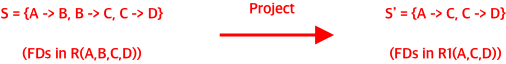
\includegraphics[width=0.7\linewidth]{images/worksheet_12_solution_2.png}
                \end{center}
            \end{itemize}

            \item Algorithm for Projecting a set of Functional Dependencies
            \begin{itemize}
                \item Inputs and Outputs
                \begin{itemize}
                    \item Input
                    \begin{itemize}
                        \item \textbf{R:} The original relation
                        \item \textbf{R1:} The projection of $R$
                        \item \textbf{S:} The set of FD's that hold in $R$
                    \end{itemize}
                    \item Output
                    \begin{itemize}
                        \item \textbf{T:} The set of $FD$'s that hold in $R_1$
                    \end{itemize}
                \end{itemize}

                \item Steps
                \begin{enumerate}[1.]
                    \item Initialize $T = \{\}$.
                    \item Construct a set of all subsets of attributes of $R_1$ called $X$
                    \item Compute $X_i^+$ for all members of $X$ under S.
                    \begin{itemize}
                        \item $X_i^+$ may consist of attributes that are not in $R1$
                    \end{itemize}
                    \item Add to $T$ all nontirival FD's $X \to A$ such that $A$
                    is both in $X_i^+$ and an attributes of $R_1$
                    \item Now, $T$ is a basis for the $FD$'s that hold in $R1$ but
                    may not be a minimal basis. Modify $T$ as follows.

                    \begin{enumerate}[a)]
                        \item If there is an $FD$ in $F$ in $T$ that follows from
                        the other $FD$'s in $T$, remove $F$
                        \item Let $Y \to B$ be an FD in $T$, with at least two
                        attributes in $Y$. Remove one attribute from $Y$ and call
                        it $Z$. If $Z \to B$ follows from the $FD$'s in $T$, then
                        replace $Z \to B$ with $Y \to B$.
                    \end{enumerate}
                \end{enumerate}
                \item Example

                \bigskip

                Consider $R(A,B,C,D)$ has $FD$'s$A \to B$, $B \to C$, and $C \to D$.

                $R_1(A,C,D)$ is a projection of $R$. Find FD's for $R_1$

                \begin{enumerate}[1.]
                    \item Initialize $T = \{\}$.
                    \color{red}
                    \begin{itemize}
                        \item $T = \{\}$
                    \end{itemize}
                    \color{black}
                    \item Construct a set of all subsets of attributes of $R_1$ called $X$
                    \color{red}
                    \begin{itemize}
                        \item There are 8 subsets

                        \bigskip

                        $X_1 = \{A\}$, $X_2 = \{C\}$, $X_3 = \{D\}$, $X_4 = \{A,C\}$,
                        $X_5 = \{A,D\}$, $X_6 = \{C,D\}$, $X_7 = \{A,C,D\}$, $X_8 = \{\}$

                    \end{itemize}
                    \color{black}
                    \item Compute $X_i^+$ for all members of $X$ under S.

                    \color{red}
                    \begin{itemize}
                        \item $X_1 = \{A\}$

                        \bigskip

                        $X_1^+ = \{A,B,C,D\}$

                        \item $X_2 = \{C\}$

                        \bigskip

                        $X_2^+ = \{C,D\}$

                        \item $X_3 = \{D\}$

                        \bigskip

                        $X_3^+ = \{D\}$

                        \item $X_4 = \{A,C\}$

                        \bigskip

                        $X_4^+ = \{A,B,C,D\}$

                        \item $X_5 = \{A,D\}$

                        \bigskip

                        $X_5^+ = \{A,B,C,D\}$

                        \item $X_6 = \{C,D\}$

                        \bigskip

                        $X_6^+ = \{C,D\}$

                        \item $X_7 = \{A,C,D\}$

                        \bigskip

                        $X_7^+ = \{A,B,C,D\}$


                        \item $X_8 = \{\}$

                        \bigskip

                        $X_8^+ = \{\}$


                    \end{itemize}
                    \color{black}

                    \item Add to $T$ all nontirival FD's $X \to A$ such that $A$
                    is both in $X_i^+$ and an attributes of $R_1$

                    \color{red}
                    \begin{itemize}
                        \item

                        $T = \{A \to C, A \to D, C \to D, AC \to D, AD \to C\}$
                    \end{itemize}
                    \color{black}

                    \item Now, $T$ is a basis for the $FD$'s that hold in $R1$ but
                    may not be a minimal basis. Modify $T$ as follows.

                    \color{red}
                    \begin{itemize}
                        \item

                        $T = \{C \to D, A \to D , A \to C\}$
                    \end{itemize}
                    \color{black}
                \end{enumerate}
            \end{itemize}
        \end{itemize}

        \item

        \begin{itemize}
            \item Finding subsets

            $X_1 = \{A\}$, $X_2 = \{B\}$, $X_3 = \{C\}$, $X_4 = \{A,B\}$, $X_5 = \{A,C\}$,
            $X_6 = \{B,C\}$, $X_7 = \{A,B,C\}$, $X_8 = \{\}$


            \item Finding $X_i^+$
            \begin{enumerate}[1.]
                \item $X_1^+ = \{A,D\}$
                \item $X_2^+ = \{B\}$
                \item $X_3^+ = \{C\}$
                \item $X_4^+ = \{A,B,D,E\}$
                \item $X_5^+ = \{A,B,C,D,E\}$
                \item $X_6^+ = \{B,C\}$
                \item $X_7^+ = \{A,B,C,D,E\}$
                \item $X_8^+ = \{\}$
            \end{enumerate}

            \item Putting all nontirival FD's in $T$

            $T = \{A \to D, AB \to D, AB \to E, AC \to B, AC \to D, AC \to E,
                   ABC \to D, ABC \to E\}$

            \item Finding minimal basis for the FD of $S$

            $T_{\text{minimal}} = \{A \to D, AB \to E, AC \to B, AC \to E\}$

        \end{itemize}

        \item

        \begin{itemize}
            \item Finding subsets

            $X_1 = \{A\}$, $X_2 = \{B\}$, $X_3 = \{C\}$, $X_4 = \{A,B\}$, $X_5 = \{A,C\}$,
            $X_6 = \{B,C\}$, $X_7 = \{A,B,C\}$, $X_8 = \{\}$


            \item Finding $X_i^+$
            \begin{enumerate}[1.]
                \item $X_1^+ = \{A\}$
                \item $X_2^+ = \{B\}$
                \item $X_3^+ = \{C\}$
                \item $X_4^+ = \{A,B,D\}$
                \item $X_5^+ = \{A,B,C,D,E\}$
                \item $X_6^+ = \{A,B,C,D,E\}$
                \item $X_7^+ = \{A,B,C,D,E\}$
                \item $X_8^+ = \{\}$
            \end{enumerate}

            \item Putting all nontirival FD's in $T$

            $T = \{AB \to D, AC \to B, AC \to D, AC \to E, BC \to A, BC \to D, BC \to E,
                   ABC \to D, ABC \to E\}$

            \item Finding minimal basis for the FD of $S$

            $T_{\text{minimal}} = \{A \to D, AC \to B, C \to A, C \to B, C \to E\}$

        \end{itemize}

        \item

        \begin{itemize}
            \item Finding subsets

            $X_1 = \{A\}$, $X_2 = \{B\}$, $X_3 = \{C\}$, $X_4 = \{A,B\}$, $X_5 = \{A,C\}$,
            $X_6 = \{B,C\}$, $X_7 = \{A,B,C\}$, $X_8 = \{\}$


            \item Finding $X_i^+$
            \begin{enumerate}[1.]
                \item $X_1^+ = \{A,B,C,D,E\}$
                \item $X_2^+ = \{A,B,C,D,E\}$
                \item $X_3^+ = \{A,B,C,D,E\}$
                \item $X_4^+ = \{A,B,C,D,E\}$
                \item $X_5^+ = \{A,B,C,D,E\}$
                \item $X_6^+ = \{A,B,C,D,E\}$
                \item $X_7^+ = \{A,B,C,D,E\}$
                \item $X_8^+ = \{\}$
            \end{enumerate}

            \item Putting all nontirival FD's in $T$

            $T = \{
                    A \to B,
                    A \to C,
                    A \to D,
                    A \to E,
                    B \to A,
                    B \to C,
                    B \to D,
                    B \to E,
                    C \to A,
                    C \to B,
                    C \to D,
                    C \to E,
                   AB \to C,
                   AB \to D,
                   AB \to E,
                   AC \to B,
                   AC \to D,
                   AC \to E,
                   BC \to A,
                   BC \to D,
                   BC \to E,
                  ABC \to D,
                  ABC \to E
                \}$

            \item Finding minimal basis for the FD of $S$

            $T_{\text{minimal}} = \{
                    A \to B,
                    A \to C,
                    A \to D,
                    A \to E,
                    B \to A,
                    B \to C,
                    B \to D,
                    B \to E,
                    C \to A,
                    C \to B,
                    C \to D,
                    C \to E
            \}$

        \end{itemize}

    \end{enumerate}

    \item

    \begin{enumerate}[a)]

        \item


        \begin{itemize}
            \item Determining BCNF violations


            \bigskip

            $\{A,B\}^+ = \{A,B,C,D\}$

            \bigskip

            $\{C\}^+ = \{A,C,D\}$ \color{red}BCNF Violations\color{black}

            \bigskip

            $\{D\}^+ = \{D,A\}$ \color{red}BCNF Violations\color{black}

            \bigskip

            \item Decomposing Relations ($C \to D$)

            \begin{enumerate}[1.]
                \item Suppose that $X \to Y$ is a BCNF violation

                \color{red}
                $C \to D$
                \color{black}

                \item Compute $X^+$ and put $R_1 = X^+$

                \color{red}
                $R_1(A,C,D)$
                \color{black}

                \item $R_2$ contain all $X$ attributes and those that are not in $X^+$

                \color{red}
                $R_2(B)$
                \color{black}

                \item Project FD's for $R_1$ and $R_2$

                \bigskip

                \begin{itemize}
                    \item $R_1$ - \color{red}$\{C \to D, C \to A, D \to A \}$\color{black}
                    \item $R_2$ - \color{red}None\color{black}

                \end{itemize}
                \item Recursively decompose $R_1$ and $R_2$

                \bigskip

                \color{red}$R_1(A,C,D):D \to A$ forms BCNF violations.\color{black}

                \bigskip

                \begin{itemize}
                    \item \color{red}Decomposition Produces $R_1 (A,D): D \to A$ and $R_2 (C)$\color{black}
                \end{itemize}


            \end{enumerate}

            \item Decomposing Relations ($D \to A$)

            \begin{enumerate}[1.]
                \item Suppose that $X \to Y$ is a BCNF violation

                \color{red}
                $D \to A$
                \color{black}

                \item Compute $X^+$ and put $R_1 = X^+$

                \color{red}
                $R_1(A,D)$
                \color{black}

                \item $R_2$ contain all $X$ attributes and those that are not in $X^+$

                \color{red}
                $R_2(B,C)$
                \color{black}

                \item Project FD's for $R_1$ and $R_2$

                \bigskip

                \begin{itemize}
                    \item $R_1(A,D)$ - \color{red}$\{D \to A\}$\color{black}
                    \item $R_2(B,C)$ - \color{red}$\{C \to D, C \to A, BC \to A, BC \to B\}$\color{black}

                \end{itemize}
                \item Recursively decompose $R_1$ and $R_2$

                \bigskip

                \color{red}$R_2(B,C): C \to D, C \to A, BC \to A, BC \to B$ forms BCNF violations.\color{black}

                \bigskip

                \begin{itemize}
                    \item \color{red}Decomposition Produces $R_1 (A,D): D \to A$ and $R_2 (C)$\color{black}
                \end{itemize}


            \end{enumerate}

        \end{itemize}


    \end{enumerate}

    \bigskip

    \underline{\textbf{Notes:}}

    \bigskip

    \begin{itemize}
        \item BCNF Form violations when closure of a a set of attributes are not complete

        \bigskip

        e.g.


        \bigskip

        $R(A,B,C,D): AB \to C, B \to D, CD \to A, AD \to B$

        \bigskip

        the above forms the following closures


        \begin{itemize}
            \item $AB^+ = \{A, B, C, D\}$
            \item $B^+ = \{B, D\}$ // this forms violations
            \item $CD^+ = \{C, D, A, B\}$
            \item $AD^+ = \{A, D, B, C\}$
        \end{itemize}

        \item Anomalies
        \begin{itemize}
            \item means ``Something that you don't expect'' in layman's terms
            \item Three main types of anomalies exist
            \begin{itemize}
                \item \textit{Redundancy} - Information may be prepeated unnecessarily in several tuples

                \bigskip

                \begin{center}
                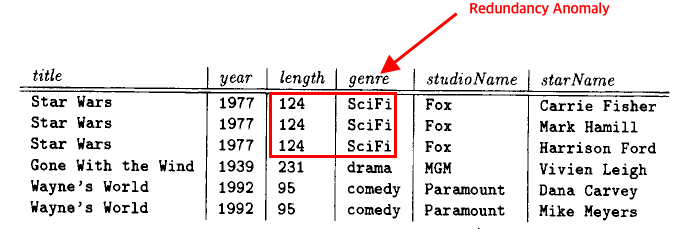
\includegraphics[width=0.7\linewidth]{images/worksheet_12_solution_3.png}
                \end{center}

                \item \textit{Update Anomalies} - information changed in one
                tuple, but the same information is not changed in the other

                \item \textit{Deletion Anomalies} - Deletion of one tuple causing
                undesired deletion of other information

                \bigskip

                e.g. deleting movie \textit{Gone with the wind} resulting
                in loss of information about studio \textit{Fox}


            \end{itemize}
        \end{itemize}

        \item Decomposing Relations
        \begin{itemize}
            \item \textit{Decompose Relations}
            \begin{itemize}
                \item is an accepted way to eliminate anomalies
                \item involves splitting the attributes of $R$ to make the schemas of two new relations.
            \end{itemize}
            \item The how of decomposing anomalies
            \begin{itemize}
                \item Given a relation $R(A_1,A_2,...,A_n)$ we may decompose
                $R$ into two relations $S(B_1, B_2, \cdots, B_m)$ and $T(C_1, C_2, \cdots, C_k)$

                \bigskip

                \begin{enumerate}[1.]
                    \item $\{A_1, A_2, \cdots, A_n\} = \{B_1, B_2, \cdots, B_m\} \cup \{C_1,C_2, \cdots, C_k\}$
                    \item $S = \pi_{B_1, B_2, \cdots, B_m}(R)$
                    \item $T = \pi_{C_1, C_2, \cdots, C_k}(R)$
                \end{enumerate}

            \end{itemize}
        \end{itemize}

        \item Boyce-Codd Normal Form
        \begin{itemize}
            \item is a simple condition under which the anormalies can be
            guarenteed NOT to exist

            \bigskip

            \begin{itemize}
                \item A relation $R$ is in BCNF if and only if: whenever there is a
                non trivial FD $A_1A_2 \cdots A_n \to B_1 B_2 \cdots B_m$ for $R$,
                it is the case that $\{A_1, A_2, \cdots A_n\}$ is a superkey for $R$.
            \end{itemize}

            \bigskip

            \underline{\textbf{Example:}}

            \begin{center}
            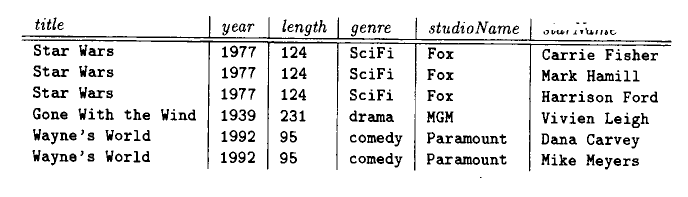
\includegraphics[width=0.7\linewidth]{images/worksheet_12_solution_4.png}
            \end{center}

            \bigskip

            Is not BCNF because 1. title year $\to$ length holds, but $\{title, year\}$
            are not superkeys

            \bigskip

            \underline{\textbf{Example 2:}}

            \bigskip

            \begin{center}
            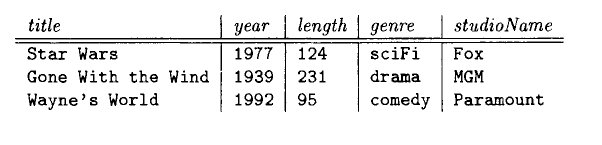
\includegraphics[width=0.7\linewidth]{images/worksheet_12_solution_5.png}
            \end{center}

            \bigskip

            In this case, the table is BCNF, because the key is $\{title, year\}$
            and no other FDs contain this key.

        \end{itemize}

        \item Decomposition into BCNF
        \begin{itemize}
            \item Fixes BCNF Violations
            \item Algorithm

            \bigskip

            \textbf{Input:} A relation $R_0$ with a set of $FD$'s $S_0$

            \bigskip

            \textbf{Output:} A decomposition of $R_0$ into a collection of relations all in $BCNF$

            \bigskip

            \begin{enumerate}[1.]
                \item Suppose that $X \to Y$ is a BCNF violation
                \item Compute $X^+$ and put $R_1 = X^+$
                \item $R_2$ contain all $X$ attributes and those that are not in $X^+$
                \item Project FD's for $R_1$ and $R_2$
                \item Recursively decompose $R_1$ and $R_2$
            \end{enumerate}

            \bigskip

            \underline{\textbf{Example:}}

            \bigskip

            e.g.


            \bigskip

            $R(A,B,C,D): AB \to C, B \to D, CD \to A, AD \to B$

            \bigskip

            the above forms the following closures

            \bigskip

            \begin{itemize}
                \item $AB^+ = \{A, B, C, D\}$
                \item $B^+ = \{B, D\}$ // this forms violations
                \item $CD^+ = \{C, D, A, B\}$
                \item $AD^+ = \{A, D, B, C\}$
            \end{itemize}

            \bigskip

            \begin{enumerate}[1.]
                \item Suppose that $X \to Y$ is a BCNF violation

                \bigskip

                \color{red}
                $B \to D$
                \color{black}

                \bigskip

                \item Compute $X^+$ and put $R_1 = X^+$

                \bigskip

                \color{red}
                $B^+ = \{B,D\} \Rightarrow R_1(B,D)$
                \color{black}

                \bigskip

                \item $R_2$ contain all $X$ attributes and those that are not in $X^+$

                \bigskip

                \color{red}
                $R_2(A,C)$
                \color{black}

                \bigskip

                \item Project FD's for $R_1$ and $R_2$

                \bigskip


                1) \color{red}For $R_1(B,D)$\color{black}

                \bigskip

                \begin{itemize}
                    \item Finding subsets

                    \bigskip
                    \color{red}

                        $X_1 = \{B\}$,
                        $X_2 = \{D\}$,
                        $X_3 = \{B,D\}$

                    \color{black}
                    \bigskip

                    \item Finding $X_i^+$

                    \bigskip
                    \color{red}

                    \begin{enumerate}[1.]
                        \item $X_1^+ = \{B\}$
                        \item $X_2^+ = \{D\}$
                        \item $X_3^+ = \{B,D\}$
                    \end{enumerate}

                    \color{black}
                    \item Putting all nontirival FD's in $T$

                    \color{red}

                    $T = \{\}$

                    \color{black}

                    \item Finding minimal basis for the FD of $S$

                    \color{red}

                    $T_{\text{minimal}} = \{\}$

                    \color{black}

                \end{itemize}

                \bigskip

                2) \color{red}$R_2(A,C)$\color{black}

                \bigskip

                \begin{itemize}
                    \item Finding subsets

                    \bigskip
                    \color{red}

                        $X_1 = \{A\}$,
                        $X_2 = \{C\}$,
                        $X_3 = \{A,C\}$

                    \color{black}
                    \bigskip

                    \item Finding $X_i^+$

                    \bigskip
                    \color{red}

                    \begin{enumerate}[1.]
                        \item $X_1^+ = \{A\}$
                        \item $X_2^+ = \{C\}$
                        \item $X_3^+ = \{A,C\}$
                    \end{enumerate}

                    \color{black}
                    \item Putting all nontirival FD's in $T$

                    \color{red}

                    $T = \{\}$

                    \color{black}

                    \item Finding minimal basis for the FD of $S$

                    \color{red}

                    $T_{\text{minimal}} = \{\}$

                    \color{black}

                \end{itemize}


                \item Recursively decompose $R_1$ and $R_2$
            \end{enumerate}


        \end{itemize}
    \end{itemize}

\end{enumerate}

\end{document}